\subsection{Negocio}

La Capa de Negocios se utiliza típicamente (en conjunto con los elementos de estrategia) para modelar la arquitectura de negocios de una empresa, definida por el marco del TOGAF como una descripción de la estructura e interacción entre la estrategia de negocios, la organización, las funciones, los procesos de negocios y las necesidades de información.

\subsubsection{Elementos de la Estructura}
\begin{table}[H]
	\centering
	\begin{tabular}{| m{3cm} | m{7cm} | m{3.8cm} |}
		\hline
		\textbf{Concepto}           & \textbf{Definición} & \textbf{Notación} \\ \hline
		
		Actor de Negocios        & Una entidad organizacional que es capaz de ejecutar un comportamiento.                                                                                                              &\vspace{1.52mm}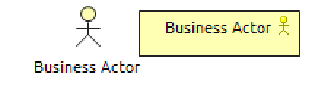
\includegraphics[width=40mm, height=10mm]{imgs/conceptos/negocio/Business_actor.pdf}    \\ \hline
		
		Rol de Negocios          & La responsabilidad de tener un comportamiento especifico, ante el cual un actor puede ser asignado.                                                                                 &\vspace{1.52mm}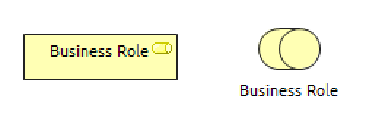
\includegraphics[width=40mm, height=10mm ]{imgs/conceptos/negocio/Business_role.pdf}         \\ \hline
		
		Colaboración de Negocios & Un agregado de dos o más roles de negocios que trabajan juntos para tener un comportamiento colectivo.                                                                             
		&\vspace{1.52mm} 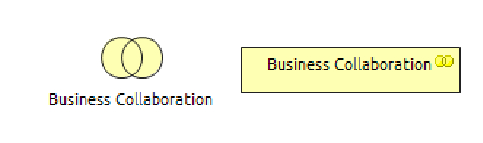
\includegraphics[width=40mm,height=10mm]{imgs/conceptos/negocio/Business_colaboration.pdf}             \\ \hline
		
		Interfaz de Negocios     & Un punto de acceso donde un servicio comercial está disponible para su entorno.                                                                                                     
		&\vspace{1.52mm}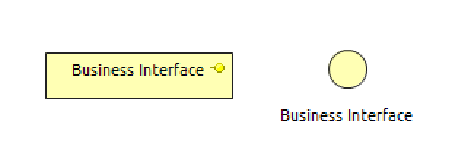
\includegraphics[width=40mm,height=10mm]{imgs/conceptos/negocio/Business_Interface.pdf}  \\ \hline
		
		Ubicación                & Un punto conceptual en el espacio.                                                                                     
		&\vspace{1.52mm}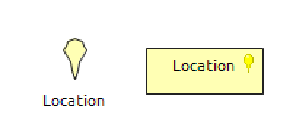
\includegraphics[width=40mm, height=10mm]{imgs/conceptos/negocio/Location.pdf}           \\ \hline
		
		Objeto de Negocios       & Un elemento pasivo que tiene relevancia desde una perspectiva de negocios.                                                                                                         
		&\vspace{1.52mm}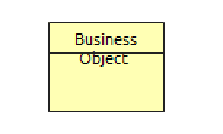
\includegraphics[width=40mm, height=10mm]{imgs/conceptos/negocio/Business_Object.pdf}   \\ \hline
		
		Proceso de Negocios      & Un elemento de comportamiento que agrupa el comportamiento basado en un orden de actividades. Es destinado a producir un  conjunto definido de productos o servicios comerciales.
		&\vspace{1.52mm} 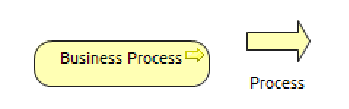
\includegraphics[width=40mm, height=10mm]{imgs/conceptos/negocio/Business_proces.pdf}            \\ \hline
		
		Función de Negocios      & Un elemento de comportamiento que agrupa el comportamiento basado en un conjunto de criterios elegidos (típicamente recursos comerciales requeridos y / o competencias).        &\vspace{1.52mm}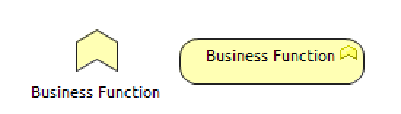
\includegraphics[width=40mm, height=10mm]{imgs/conceptos/negocio/Business_function.pdf}            \\ \hline
		
		Interacción de Negocios  & Un elemento de comportamiento que describe la conducta de una colaboración empresarial.                                                                                             
		&\vspace{1.52mm} 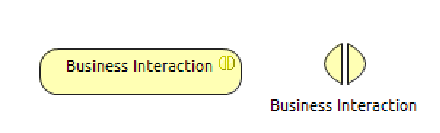
\includegraphics[width=40mm,height=10mm]{imgs/conceptos/negocio/Business_interaction.pdf}            \\ \hline
		
		Evento de Negocios       & Algo que sucede (internamente o externamente) e influye en el  comportamiento.                                                                                                       
		&\vspace{1.52mm} 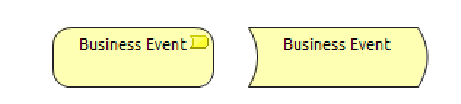
\includegraphics[width=40mm, height=10mm]{imgs/conceptos/negocio/Business_event.pdf}  \\ \hline
		
	\end{tabular}
\end{table}

\newpage
\begin{table}[H]
	\centering
	\begin{tabular}{| m{3cm} | m{7cm} | m{3.8cm} |}
		\hline
		\textbf{Concepto}           & \textbf{Definición} & \textbf{Notación} \\ \hline
		
		Servicio de Negocios     & Un servicio que satisface una necesidad comercial de un cliente (interno o externo al organización).        &\vspace{2mm}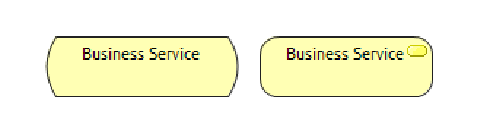
\includegraphics[width=40mm, height=8mm]{imgs/conceptos/negocio/Business_service.pdf}  \\ \hline
		
		Representación           & Una forma perceptible de la información llevado por un objeto de negocios.                                                                                                           &\vspace{1.52mm}  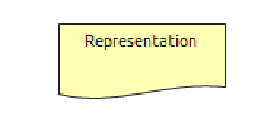
\includegraphics[width=40mm, height=10mm]{imgs/conceptos/negocio/Representation.pdf}            \\ \hline
		Significado              & El conocimiento o experiencia presente en un objeto de negocios o su representación, dado un contexto particular.                                                                   &\vspace{1.52mm}
\includegraphics[width=40mm, height=8mm]{imgs/conceptos/negocio/Meaning.pdf}           \\ \hline
		
		Valor                    & El valor relativo, la utilidad o la importanciade un servicio o producto comercial.                                                                                                  
		&\vspace{1.52mm}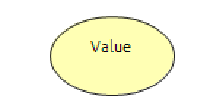
\includegraphics[width=40mm, height=10mm]{imgs/conceptos/negocio/Value.pdf}        \\ \hline
		
		Producto                 & Una colección coherente de servicios, acompañado de un contrato / conjunto de acuerdos, que se ofrece en su conjunto para (internos o externos) clientes.                           &\vspace{1.52mm}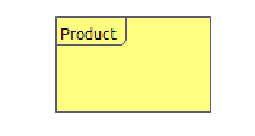
\includegraphics[width=40mm, height=10mm]{imgs/conceptos/negocio/Product.pdf}         \\ \hline
		
		Contrato                 & Una especificación formal o informal de acuerdo que especifica los derechos y obligaciones asociadas con un producto.                                                                 &\vspace{1.52mm}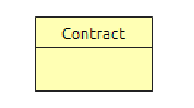
\includegraphics[width=40mm, height=10mm]{imgs/conceptos/negocio/Contract.pdf}       \\ \hline
		
	\end{tabular}
\end{table}